%%%
%%%  VZOR PRO VYTVOŘENÍ BAKALÁŘSKÉ PRÁCE 
%%%  
%%%  * soubor obsahující fiktivní třetí kapitolu
%%%
%%%  AUTOŘI:  Arnošt Komárek (komarek@karlin.mff.cuni.cz), 2011
%%%           Michal Kulich (kulich@karlin.mff.cuni.cz), 2013
%%%
%%%  POSLEDNÍ ÚPRAVA: 20130315
%%%  
%%%  ===========================================================================

\chapter{Tabulky, obrázky, softwarový kód}

Používání tabulek a grafů v~odborném textu má některá společná
pravidla a~některá specifická. Tabulky a grafy neuvádíme přímo do
textu, ale umístíme je buď na samostatné stránky nebo na vyhrazené
místo v~horní nebo dolní části běžných stránek. \LaTeX\ se o~umístění
plovoucích grafů a tabulek postará automaticky. Každý graf a tabulku
očíslujeme a umístíme pod ně legendu. Legenda má popisovat obsah grafu
či tabulky tak podrobně, aby jim čtenář rozuměl bez důkladného
studování textu práce. Na každou tabulku a graf musí být v~textu odkaz
pomocí jejich čísla. Na příslušném místě textu pak shrneme ty
nejdůležitější závěry, které lze z~tabulky či grafu učinit. Text by
měl být čitelný a srozumitelný i~bez prohlížení tabulek a grafů a
tabulky a grafy by měly být srozumitelné i~bez podrobné četby textu.
Na tabulky a grafy odkazujeme pokud možno nepřímo v~průběhu běžného
toku textu; místo \emph{\uv{Tabulka~\ref{tab03:Nejaka} ukazuje, že
    muži jsou v~průměru o~$9,9$ kg těžší než ženy}} raději napíšeme
\emph{\uv{Muži jsou o~$9,9$ kg těžší než ženy (viz
    Tabulka~\ref{tab03:Nejaka})}}.

%%%%% ===============================================================================
\section{Tabulky}


\begin{table}[b!]
  \caption{Maximálně věrohodné odhady v~modelu M.}\label{tab03:Nejaka}

\centering
%%% Tabulka používá následující balíčky:
%%%   - booktabs (\toprule, \midrule, \bottomrule)
%%%   - dcolumn (typ sloupce D: vycentrovaná čísla zarovnaná na
%%%     desetinnou čárku
%%%     Všimněte si, že ve zdrojovém kódu jsou desetinné tečky, ale
%%%     tisknou se čárky.
%%% Dále používáme příkazy \pulrad a \mc definované v BcPrace.tex

\begin{tabular}{l@{\hspace{1.5cm}}D{.}{,}{3.2}D{.}{,}{1.2}D{.}{,}{2.3}}
  \toprule
  & \mc{} & \mc{\textbf{Směrod.}} & \mc{} \\
\pulrad{\textbf{Efekt}} & \mc{\pulrad{\textbf{Odhad}}} & \mc{\textbf{chyba}$^a$} & 
\mc{\pulrad{\textbf{P-hodnota}}} \\
\midrule
Abs. člen     & -10.01 & 1.01 & \mc{---} \\
Pohlaví (muž) & 9.89   & 5.98 & 0.098 \\
Výška (cm)    & 0.78   & 0.12 & <0.001 \\ 
\bottomrule
\multicolumn{4}{l}{\footnotesize \textit{Pozn:} 
$^a$ Směrodatná chyba odhadu metodou Monte Carlo.}
\end{tabular}


\end{table}


U~\textbf{tabulek} se doporučuje dodržovat následující pravidla:
\begin{compactitem} %% vyžaduje balík paralist
\item Vyhýbat se svislým linkám. Silnějšími vodorovnými linkami
  oddělit tabulku od okolního textu včetně legendy, slabšími
  vodorovnými linkami oddělovat záhlaví sloupců od těla tabulky a
  jednotlivé části tabulky mezi sebou. V~\LaTeX u tuto podobu tabulek
  implementuje balík \texttt{booktabs}. Chceme-li výrazněji oddělit
  některé sloupce od jiných, vložíme mezi ně větší mezeru.
\item Neměnit typ, formát a význam obsahu políček v~tomtéž sloupci
  (není dobré do téhož sloupce zapisovat tu průměr onde procenta).
\item Neopakovat tentýž obsah políček mnohokrát za sebou. Máme-li
  sloupec \textit{Rozptyl}, který v~prvních deseti řádcích obsahuje
  hodnotu 0.5 a v~druhých deseti řádcích hodnotu 1.5, pak tento
  sloupec raději zrušíme a vyřešíme to jinak. Například můžeme tabulku
  rozdělit na dvě nebo do ní vložit popisné řádky, které informují
o~nějaké proměnné hodnotě opakující se v~následujícím oddíle tabulky
  (např. \emph{\uv{Rozptyl $=$ 0.5}} a níže \emph{\uv{Rozptyl $=$
      1.5}}).
\item Čísla v~tabulce zarovnávat na desetinnou tečku.
\item V~tabulce je někdy potřebné používat zkratky, které se jinde
nevyskytují. Tyto zkratky můžeme vysvětlit v~legendě nebo
v~poznámkách pod tabulkou. Poznámky pod tabulkou můžeme využít i
k~podrobnějšímu vysvětlení významu  některých sloupců nebo hodnot.
\end{compactitem}




\section{Obrázky}

Několik rad týkajících se obrázků a grafů.
\begin{compactitem}
\item Graf by měl být vytvořen ve velikosti, v~níž bude použit
  v~práci. Zmenšení příliš velkého grafu vede ke špatné čitelnosti
  popisků.
\item Osy grafu musí být řádně popsány ve stejném jazyce, v~jakém je
  psána práce (absenci diakritiky lze tolerovat). Kreslíme-li graf
  hmotnosti proti výšce, nenecháme na nich popisky \texttt{ht} a
  \texttt{wt}, ale osy popíšeme \emph{Výška [cm]} a~\emph{Hmotnost
    [kg]}. Kreslíme-li graf funkce $h(x)$, popíšeme osy $x$ a $h(x)$.
  Každá osa musí mít jasně určenou škálu.
\item Chceme-li na dvourozměrném grafu vyznačit velké množství bodů,
  dáme pozor, aby se neslily do jednolité černé tmy. Je-li bodů mnoho,
  zmenšíme velikost symbolu, kterým je vykreslujeme, anebo vybereme
  jen malou část bodů, kterou do grafu zaneseme. Grafy, které obsahují
  tisíce bodů, dělají problémy hlavně v~elektronických dokumentech,
  protože výrazně zvětšují velikost souborů.
\item Budeme-li práci tisknout černobíle, vyhneme se používání barev.
  Čáry rozlišujeme typem (plná, tečkovaná, čerchovaná,\ldots), plochy
  dostatečně rozdílnými intensitami šedé nebo šrafováním. Význam
  jednotlivých typů čar a~ploch vysvětlíme buď v~textové legendě ke
  grafu anebo v~grafické legendě, která je přímo součástí obrázku.
\end{compactitem}

Pomocí příkazu \texttt{{\textbackslash}psfrag} lze nahrazovat části
\textsf{ps/eps} souborů (typicky popisky v~obrázcích) libovolnou
kombinací {\LaTeX}ových příkazů, jak ukazují následující příklady.



\begin{figure}[ht]\centering
  \psfrag{x}[c][c]{\textsf{\large horizontální osa ($\mu_1 = 0, \sigma_1^2 = 1$)}}
  \psfrag{y}[c][c]{\textsf{\large vertikální osa ($\mu_2 = 0, \sigma_2^2 = 1$)}}
  \psfrag{Plot}[c][c]{\textsf{\bfseries\Large Bodový graf}}
  
  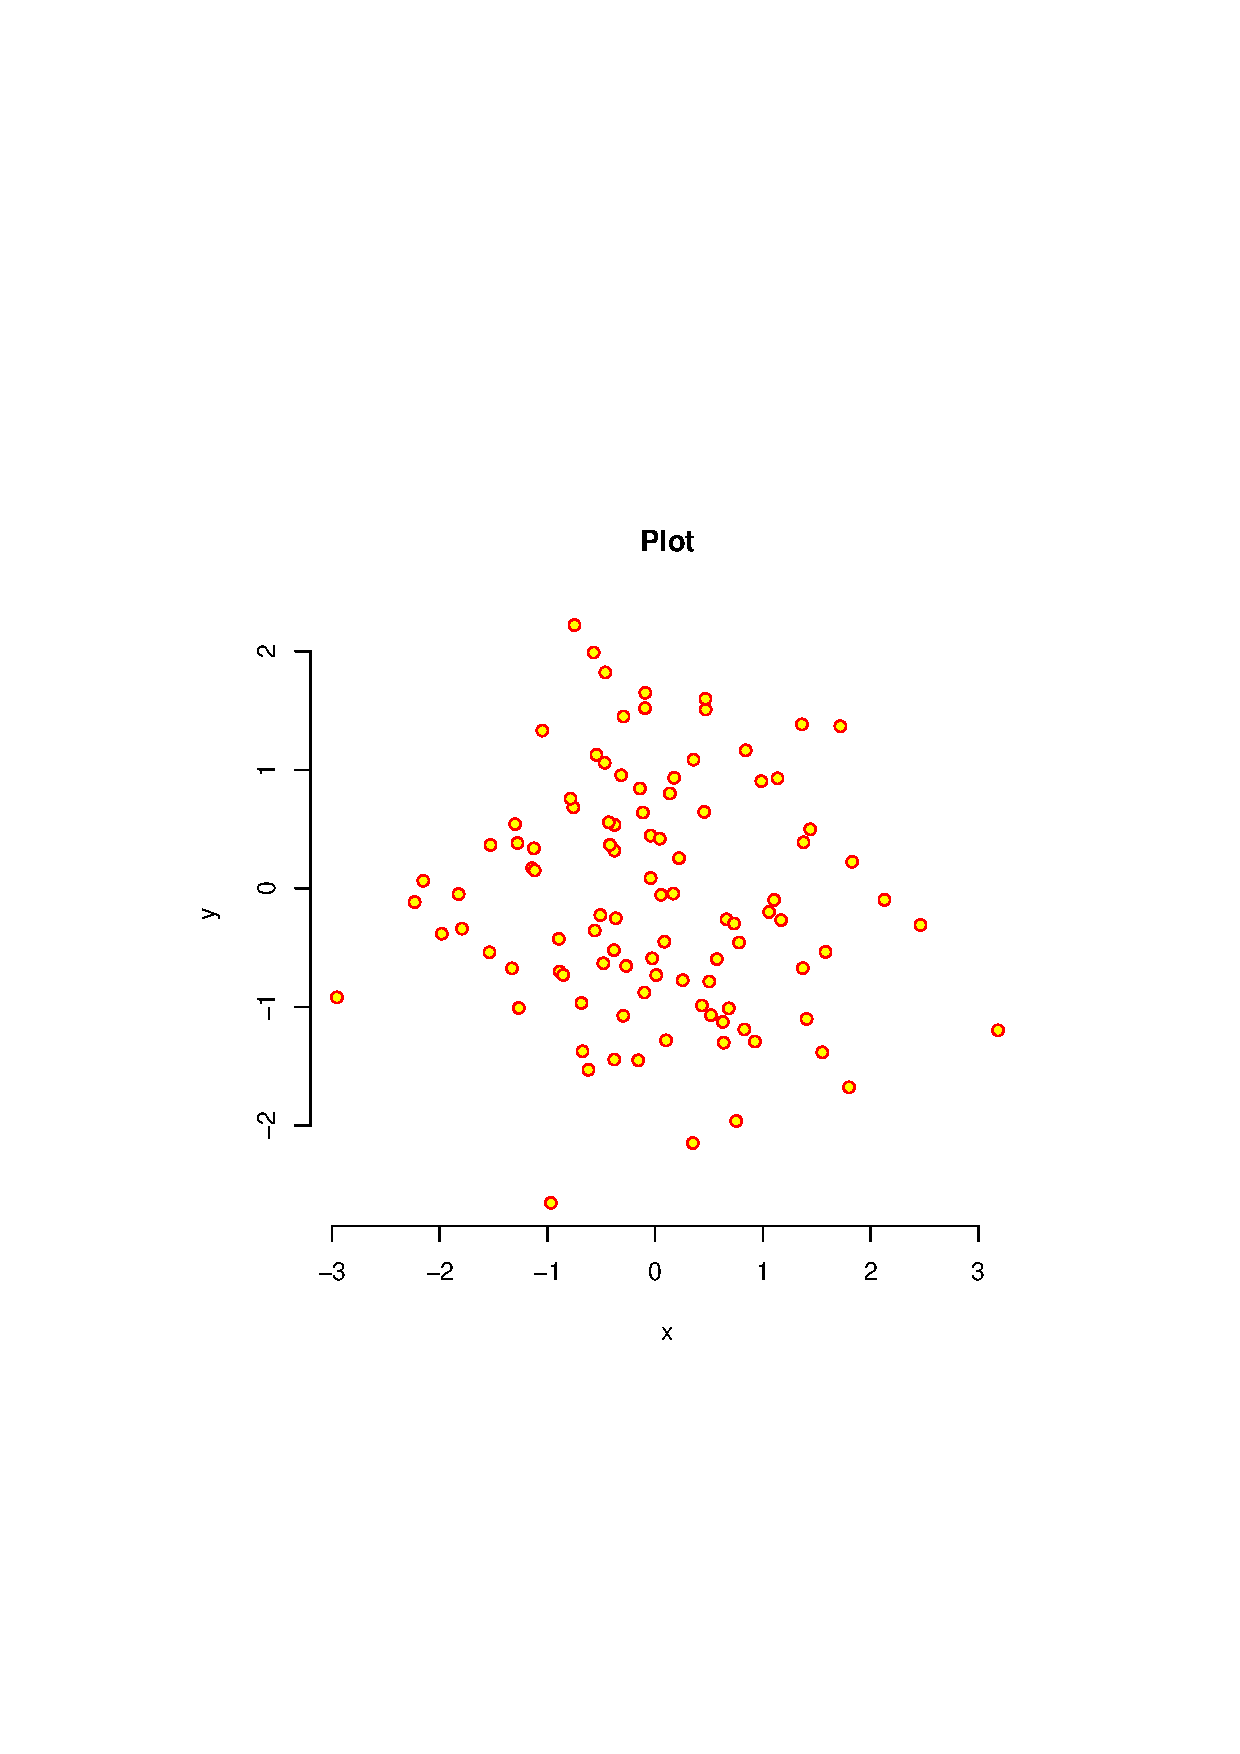
\includegraphics[width=6in, height=6in]{\FIGDIR/obr01}     
  %% příponu není potřeba explicitně uvádět, latex automaticky hledá
  %% ps/eps, pdflatex automaticky hledá pdf psfrag funguje pouze s
  %% ps/eps obrázky 
  
  \caption{Náhodný výběr z~rozdělení $\mathcal{N}_2(\boldsymbol{0},\,I)$.}
  \label{obr03:Nvyber}
  
  \end{figure}
  
  
  \begin{figure}[ht]\centering
  \label{obr03:Nhust}

  \psfrag{0.00}[c][c]{\textsf{0{,}00}}  
  \psfrag{0.02}[c][c]{\textsf{0{,}02}}  
  \psfrag{0.04}[c][c]{\textsf{0{,}04}}
  \psfrag{0.06}[c][c]{\textsf{0{,}06}}  
  \psfrag{0.08}[c][c]{\textsf{0{,}08}}
  \psfrag{m = 100, s = 15}[l][l]{\textsf{\large $\mu = 100,\; \sigma = 15$}}
  \psfrag{m = 110, s = 10}[l][l]{\textsf{\large $\mu = 110,\; \sigma = 10$}}
  \psfrag{m = 120, s = 5}[l][l]{\textsf{\large $\mu = 120,\; \sigma = 5$}}
  
  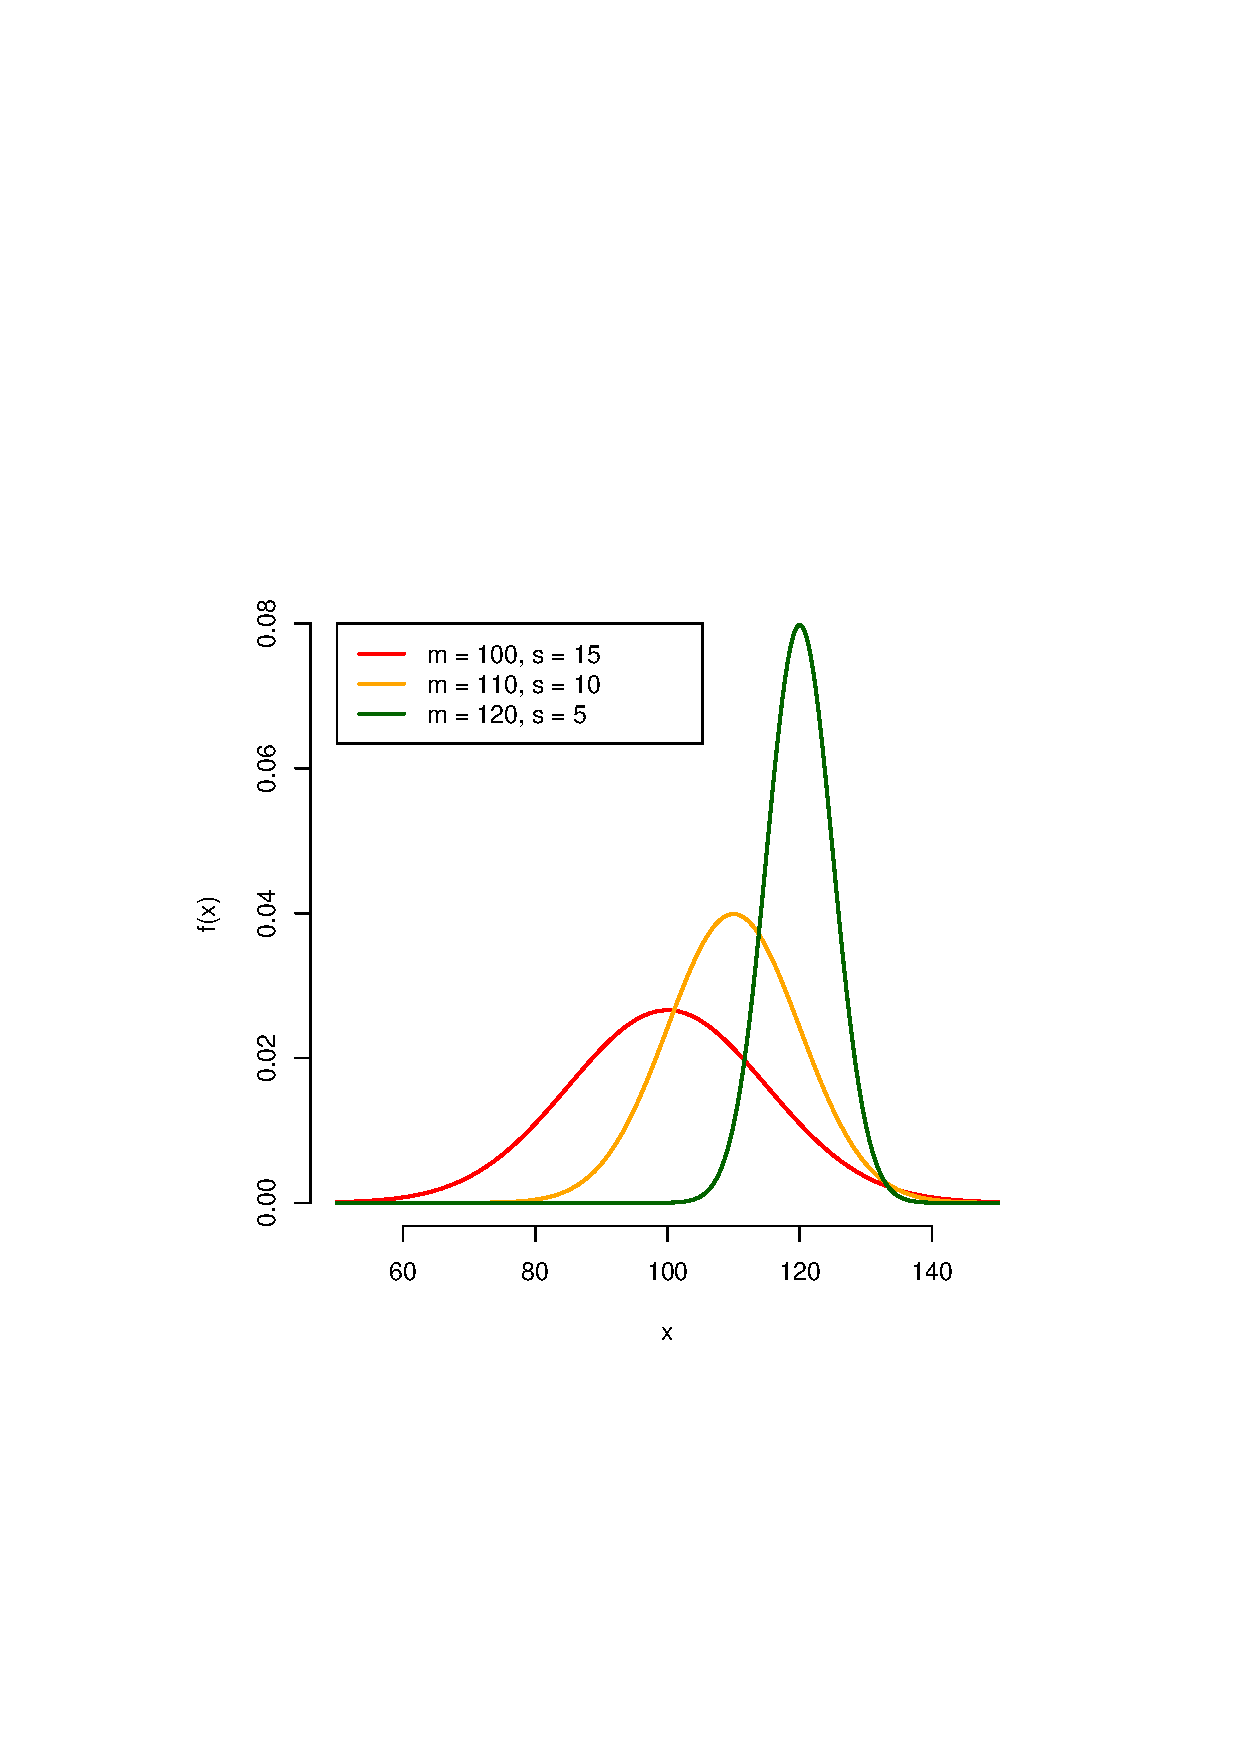
\includegraphics[width=6in, height=6in]{\FIGDIR/obr02}
  
  \caption{Hustoty několika normálních rozdělení.}
  
  \end{figure}
  
  
  % \begin{figure}[h]\centering
  % \psfrag{0.00}[c][c]{\textsf{\small 0{,}00}}  
  % \psfrag{0.02}[c][c]{\textsf{\small 0{,}02}}  
  % \psfrag{0.04}[c][c]{\textsf{\small 0{,}04}}
  % \psfrag{0.06}[c][c]{\textsf{\small 0{,}06}}  
  % \psfrag{0.08}[c][c]{\textsf{\small 0{,}08}}
  % \psfrag{60}[c][c]{\textsf{\small 60}}    
  % \psfrag{80}[c][c]{\textsf{\small 80}}  
  % \psfrag{100}[c][c]{\textsf{\small 100}}
  % \psfrag{120}[c][c]{\textsf{\small 120}}  
  % \psfrag{140}[c][c]{\textsf{\small 140}}
  % \psfrag{f\(x\)}[c][c]{\textsf{\small f(x)}}      
  % \psfrag{x}[c][c]{\textsf{\small x}}
  % \psfrag{m = 100, s = 15}[l][l]{\textsf{\large $\boldsymbol{\mu} \mathbf{\;= 100,}\; \boldsymbol{\sigma} \mathbf{\;= 15}$}}
  % \psfrag{m = 110, s = 10}[l][l]{\textsf{\large $\boldsymbol{\mu} \mathbf{\;= 110,}\; \boldsymbol{\sigma} \mathbf{\;= 10}$}}
  % \psfrag{m = 120, s = 5}[l][l]{\textsf{\large $\boldsymbol{\mu}  \mathbf{\;= 120,}\; \boldsymbol{\sigma} \mathbf{\;= 5}$}}
  
  % 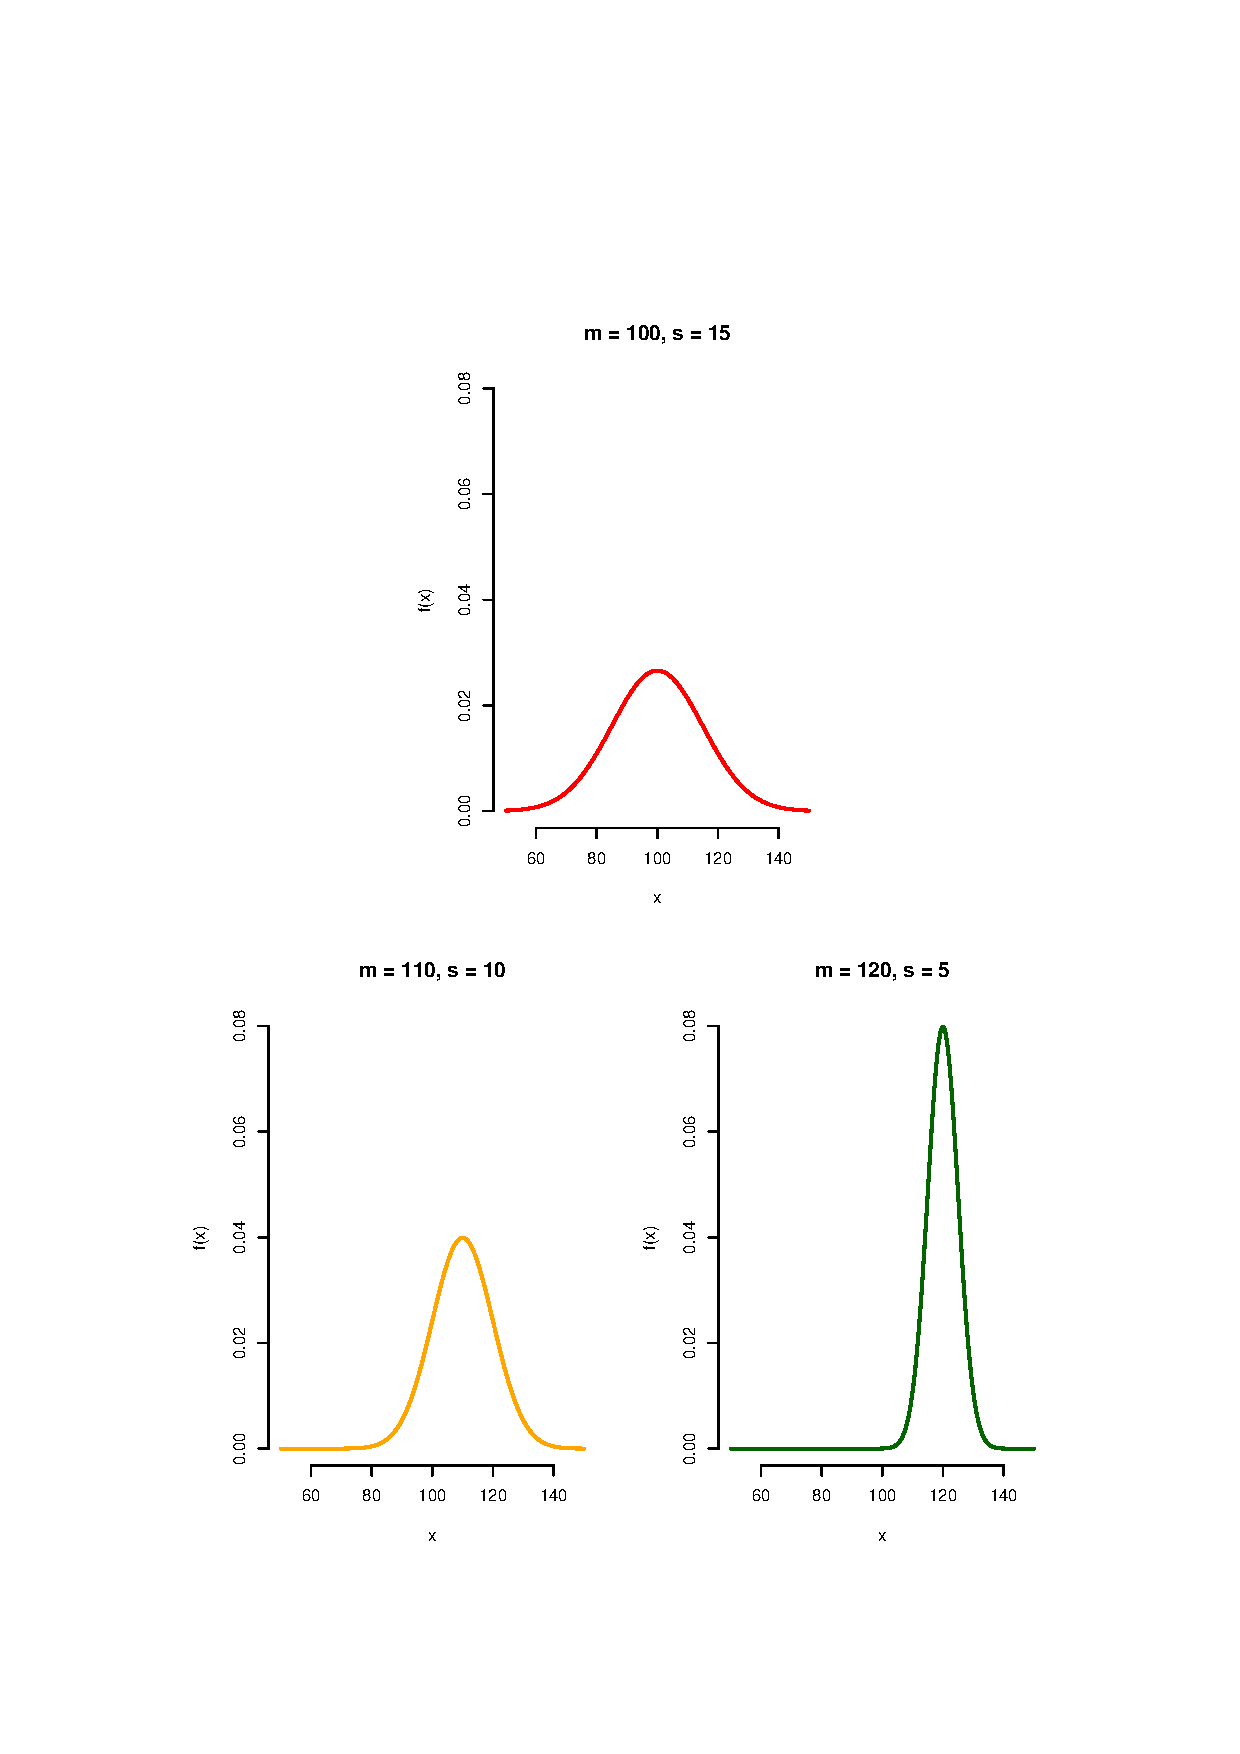
\includegraphics[width=6in, height=8.5in]{\FIGDIR/obr03}
  
  % \caption{Hustoty několika normálních rozdělení.}
  % \label{obr03:Nhust:podruhe}
  
  % \end{figure}




\section{Softwarový kód}

Softwarový kód, resp. výstupy z~počítačových programů (je-li potřeba
je v~práci uvádět) je vhodné odlišit od ostatního textu. Jednou
z~možností je použití {\LaTeX}o\-vé\-ho balíčku \texttt{fancyvrb}
(fancy verbatim), pomocí něhož je v~souboru \texttt{BcPrace.tex}
nadefinováno prostředí \texttt{PCinout}. Pomocí něho lze vytvořit
např. následující ukázky.
\begin{PCinout}
> mean(x)
[1] 158.90
> objekt\$prumer
[1] 158.90
\end{PCinout}
%$
Menší písmo:
\begin{PCinout}[fontsize=\footnotesize]
> mean(x)
[1] 158.90
> objekt\$prumer
[1] 158.90
\end{PCinout}
%$
Bez rámečku:
\begin{PCinout}[frame=none]
> mean(x)
[1] 158.90
> objekt\$prumer
[1] 158.90
\end{PCinout}
%$
Užší rámeček:
\begin{PCinout}[xrightmargin=20em]
> mean(x)
[1] 158.90
> objekt\$prumer
[1] 158.90
\end{PCinout}
%$



\newpage
\section{ukazka kodu}
\begin{lstlisting}
  class cell:
  ...
      def force_scalar(self, distance_between, direction, effect = True):
          epsilon = 0.0103
          sigma = 3.4
          return (48 * epsilon * np.power(sigma, 12) / np.power(distance_between, 13) - 24 * epsilon * np.power(sigma, 6) / np.power(distance_between, 7) * effect) * direction

      def energy_potential(self, distance_between, effect = True):
          epsilon = 0.0103
          sigma = 3.4
          return -4 * epsilon * np.power(sigma / distance_between, 6) * effect + 4 * epsilon * np.power(sigma / distance_between, 12)

      def find_centroid(self):
          # nalezeni teziste bunky, celkove hmotnosti a charakteru
          self.neutrals = 0
          self.particles_type = 0
          self.effect = 0
          self.N_particles = len(self.particles)
          if self.N_particles > 0:
              self.mass = 0
              self.centroid = np.array([0.0, 0.0, 0.0])
              for particle in self.particles:
                  self.centroid += particle.xyz*particle.mass
                  self.mass += particle.mass
                  self.particles_type += particle.particle_type
                  if particle.particle_type == 0:
                      self.neutrals += 1
              if self.particles_type != 0:
                  self.effect = self.particles_type / abs(self.particles_type)
              else:
                  self.effect = 0
              self.centroid = self.centroid/self.mass
          else:
              self.centroid = np.array([0.0, 0.0, 0.0])
              self.mass = 0
\end{lstlisting}
